\documentclass[9pt,a4paper]{extarticle}

\usepackage{f1000_styles}

\usepackage{hyperref}

\usepackage[numbers]{natbib}

\usepackage{tcolorbox} % for \texttt{}

\usepackage{bbding} % for \CheckmarkBold

% include \verb macros in \caption of figures

% http://tex.stackexchange.com/a/8814

\usepackage{cprotect}

\begin{document}

\pagestyle{front}

\title{CREATING AND SHARING REPRODUCIBLE RESEARCH CODE THE WORKFLOWR
WAY}

\author[1]{John D. Blischak}

\author[1,2]{Peter Carbonetto}

\author[1,3]{Matthew Stephens}

\affil[1]{Department of Human Genetics, University of Chicago}

\affil[2]{Research Computing Center, University of Chicago}

\affil[3]{Department of Statistics, University of Chicago}

\maketitle

\thispagestyle{front}

\begin{abstract}

\# Note: Abstract can be as long as 300 words.

The workflowr R package helps scientists create code and results that
are organized, reproducible, well-documented, and more effectively
communicated with other scientists. Workflowr provides a core set of
commands that are easily integrated into research practice to make
projects more reproducible and accessible. The core workflowr commands
implement four key features of reproducible code: (1) an automatic
project structure is provided that promotes better organization of data,
code and results; (2) new results, and the code used to generate them,
are incorporated into a project development history; (3)
"reproducibility checks" accompany each collection of code and results;
and (4) additional tools facilitate online sharing of the project and
its development history. To achieve these reproducibility features,
workflowr integrates version control (Git), literate programming tools
(knitr, R Markdown) and static website hosting (e.g., GitHub Pages) into
a simple, uniform interface in R. Our aim is to encourage all
scientists, regardless of background, to develop reproducible research
code, and share it. The workflowr R package is open source and available
on CRAN, with full documentation and source code available at
https://github.com/jdblischak/workflowr.

\end{abstract}

\section*{Keywords}

reproducibility, open science, workflow, R, interactive programming,
literate programming, version control

\clearpage

\pagestyle{main}


\section*{Introduction}

A central tenet of the scientific method is that results should be
independently verifiable --- and, ideally, extendible --- by other
researchers. As computational methods play an increasing role in many
disciplines, key scientific results are often produced by computer code.
Verifying and extending such results requires that the code be
``reproducible''; that is, it can be accessed and run, with outputs that
can be corroborated against published results \cite{Buckheit1995,
Gentleman2005, Peng2011, Ince2012, Morin2012, Sandve2013,
Easterbrook2014, Stodden2016, Lowndes2017}. Unfortunately, this ideal is
not usually achieved in practice; most scientific articles do not come
with code that can reproduce their results \cite{Ioannidis2009,
Ioannidis2014, Stodden2018}.

There are many barriers to sharing reproducible code and corresponding
computational results. One barrier is simply that keeping code and
results sufficiently organized and documented is difficult --- it is
burdensome even for experienced programmers who are well-trained in
relevant computational tools such as version control (discussed later),
and even harder for the many domain scientists who write code with
little formal training in computing and informatics \cite{Wilson2014}.
Further, modern interactive computer environments (e.g., R, python),
while greatly enhancing code development \cite{Findler2002}, also make
it easier to create results that are irreducible. To take one example,
it is all too easy to run interactive code without recording or
controlling the seed of a pseudo-random number generator, or generate
results in a ``contaminated'' environment that contains objects whose
values are critical but unrecorded. Both these issues can lead to
results that are difficult or impossible to reproduce. Finally, even
when analysts produce code that is reproducible in principle, sharing it
in a way that makes it easy for others to retrieve and use (e.g., via
GitHub or Bitbucket) involves technologies that many scientists are not
familiar with \cite{Marwick2017, Stodden2018}.

In light of this, there is a pressing need for easy-to-use tools to help
analysts maintain reproducible code, document progress, and disseminate
code and results to collaborators, and to the scientific community. We
have developed an open source R \cite{R2019} package, "workflowr", to
address this need. The workflowr package aims to instill a particular
"workflow" --- a sequence of steps to be repeated and integrated into
research practice --- that helps make projects more reproducible and
accessible. To achieve this, workflowr integrates four key features that
facilitate reproducible code development: (1) version control
\cite{Loeliger2012, Chacon2014}; (2) literate programming
\cite{Xie2018}; (3) simple automated safeguards such as setting and
recording the random number seed that improve code reproducibility,
which are reported as a series of "reproducibility checks"; and (4)
sharing code and results via a browsable website. These features exploit
powerful existing tools, whose mastery would take considerable study.
However, the workflowr interface is designed to be simple so that
learning it does not become another barrier in itself, and novice users
can quickly enjoy its many benefits. By simply following the "workflowr
workflow", R users can create projects whose results and figures are
easily accessible on a static website --- thereby conveniently shareable
with collaborators by sending them a URL --- and accompanied by source
code and reproducibility safeguards. The Web-based interface, updated
with version control, also makes it easy to navigate through different
parts of the project and browse the project history, including previous
versions of figures and results, and the code used to produce them. When
using workflowr, all this can be achieved with minimal experience in
version control systems and Web technologies.

The workflowr package builds on several software technologies and R
packages, without which this work would have been impossible. First,
workflowr builds on the invaluable R Markdown literate programming
system implemented in knitr \cite{Xie2014, knitr} and rmarkdown
\cite{Xie2018, rmarkdown}, which in turn build on pandoc, the "Markdown"
markup language, and various Web technologies such as Cascading Style
Sheets and Bootstrap \cite{Spurlock2013}. Several popular R packages
extend knitr and rmarkdown for specific uses such as writing blogs
(blogdown), monographs (bookdown) and software documentation (pkgdown).
Analogously, workflowr augments rmarkdown with additional features such
as the reproducibility safeguards, and adds integration with Git. Git
was designed to support large-scale, distributed software development,
but in workflowr it serves a different purpose: to record, and provide
access to, the development history of a project. Workflowr also uses
another Git feature, "remotes", to enable collaborative project
development across multiple locations, and to help users create
browsable projects via integrations with popular online services such as
GitHub Pages and GitLab Pages. These features are implemented using the
R package git2r, which provides an interface to the libgit2 C library.
Finally, beyond extending the R programming language, workflowr is also
integrated seamlessly with the popular RStudio interactive development
environment.

In addition to the tools upon which workflowr directly builds, there are
many other related tools that directly or indirectly advance open and
reproducible data analysis. A comprehensive review of such tools is
beyond the scope of this article, but we note that many of these tools
are complementary to workflowr in that they tackle aspects of
reproducibility that workflowr currently leaves to the user, such as:
management and deployment of computational environments and dependencies
(e.g., conda, Homebrew, Singularity, Docker, Kubernetes, packrat,
checkpoint, switchr, RSuite); development and management of
computational pipelines (e.g., GNU Make, Snakemake, drake); management
and archival of data objects (e.g., archivist, cacher, Dryad, Zenodo);
and distribution of open source software (e.g., CRAN, Bioconductor,
Bioconda). Most of these tools or services could be used in combination
with workflowr. There are additional, very ambitious efforts to develop
cloud-based services that come with many computational reproducibility
features (e.g., Code Ocean, Binder, Gigantum, The Whole Tale). Many of
these platforms manage individual projects as Git repositories, so
workflowr could, in principle, be installed and used on these platforms,
possibly to enhance their existing features. Other R packages with
utilities to facilitate reproducibility that could complement workflowr
include ProjectTemplate, rrtools and usethis, as well as many of the R
packages listed in the "Reproducible Research" CRAN Task View
(https://CRAN.R-project.org/view=ReproducibleResearch) and our own
(unofficial) Task View on "Project Workflows"
(https://github.com/jdblischak/ctv-project-workflows).

Of the available software tools facilitating reproducible research,
perhaps the closest in scope to workflowr are the R package adapr
\cite{Gelfond2018} and the Python-based toolkit Sumatra
\cite{Davidson2014}. Like workflowr, both adapr and Sumatra use version
control to maintain a project development history. Unlike workflowr,
both place considerable emphasis on managing and keeping track of
dependencies (software and data), whereas workflowr only records this
information. In contrast, workflowr places more emphasis on literate
programming --- the publishing of text and code in a readable form ---
and more closely integrates other features such as tracking project
development history via Git with literate programming.

The workflowr R package is available from CRAN
(https://cran.r-project.org/package=workflowr) and GitHub
(https://github.com/jdblischak/workflowr), and is distributed under the
flexible open source MIT license. Extensive documentation, tutorials and
user support can be found at the GitHub site. In the remainder of this
article, we describe the workflowr interface, explain its design, and
give examples illustrating how workflowr is used in practice (see "Use
Cases").


\section*{Methods}

The workflowr R package makes data analysis projects more organized,
tracked, reproducible, and shareable. The R package and its dependencies
are straightforward to install, while also being highly customizable for
more dedicated users. In the following sections, we give an overview of
the features of the workflowr R package, and describe their
implementation. For step-by-step instructions on starting a workflowr
project, see the
\href{https://jdblischak.github.io/workflowr/articles/wflow-01-getting-started.html}{"Getting
started with workflowr"} vignette.

\subsection*{Operation}

For basic usage, only five functions are needed:

\begin{itemize}

\item \texttt{wflow\_start()} initializes a new project, including the template
directory structure (Figure 1A);

\item \texttt{wflow\_build()} renders the webpages from the Rmd analysis files,
with reproducibility safeguards in place;

\item \texttt{wflow\_publish()} commits the rendered webpages --- and the code
that generated these webpages --- to the project development history;

\item \texttt{wflow\_status()} is used to check the status of the project files;
and

\item \texttt{wflow\_git\_push()} uploads the results from the user's local
repository to a website hosting service.

\end{itemize}

\textit{The primary output of workflowr is a project website for
browsing the results generated by the Rmd analysis files} (Figure 1B).
The use of websites to organize information is, of course, now
widespread. Nonetheless, we believe they are under-utilized for
organizing results of scientific projects. In particular hypertext
provides an ideal way to connect different analyses that have been
performed, and to provide easy access to relevant external data (e.g.
related work or helpful background information); see Figure \ref{fig:organized}B, and Use
Cases for examples).

\subsubsection*{Organizing the project: \texttt{wflow\_start()}}



\begin{figure}

\# Figure \ref{fig:organized}

\centering

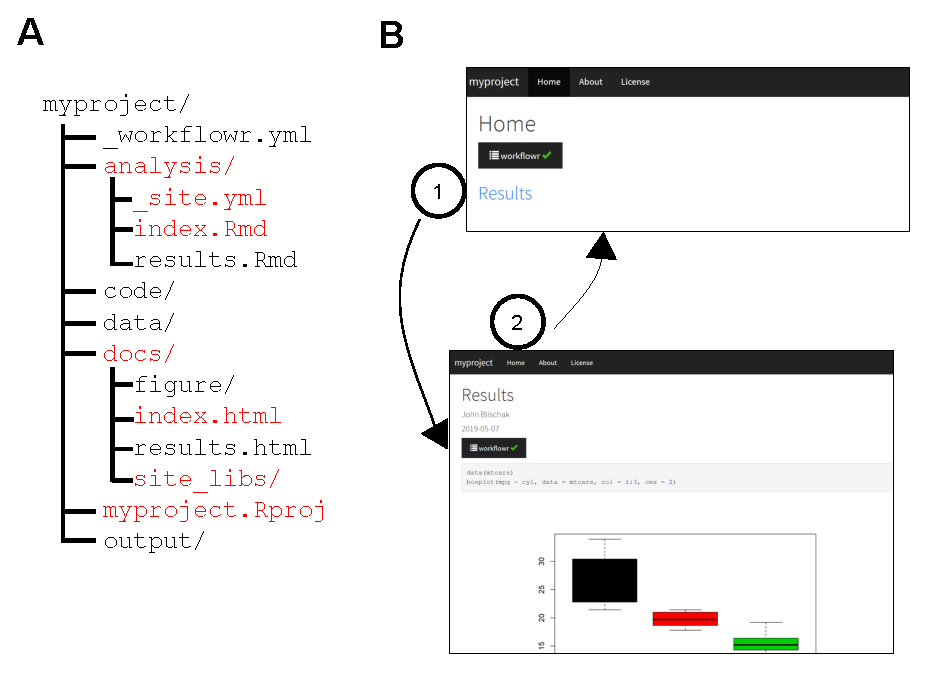
\includegraphics[width=0.8\textwidth]{figures/wflow-fig-1-v01.eps}

\cprotect\caption{\label{fig:organized}

The workflowr package helps organize files and results. A) The function
\texttt{wflow\_start()} populates a project directory with all the files needed to
begin a workflowr project. The default directory structure encourages
users to organize their files as the project progresses. (This is only a
suggested structure, and users may change the names of many of these
files and directories.) Files required by workflowr are depicted in red.
B) All results are organized into a website which is stored within the
project directory (in \texttt{docs/}). The use of hyperlinks allows for
efficient access of the results. The example screenshots illustrate how
a workflowr website can be navigated. Clicking a hyperlink in the main
page (1) navigates the browser to a webpage containing some results;
clicking on the "Home" hyperlink (2) in the navigation bar brings the
browser back to the main page.

}

\end{figure}

The function \texttt{wflow\_start()} facilitates project organization by
populating a directory with suggested subdirectories, scripts, and
configuration files for a data analysis project (Figure \ref{fig:organized}A). The
subdirectories include by default: analysis/ , where the Rmd analysis
files are stored; docs/, which stores the website HTML files; code/,
which is intended for longer-running scripts, compiled code (e.g., C++)
and other source code supporting the data analyses; data/, for storing
raw data files; and output/ for saving processed data files and other
outputs generated by the scripts and analyses. This setup is flexible
and configurable; only two of these directories, \verb|analysis/| and
\verb|docs/|, are required, and both can be renamed later.

\subsubsection*{Generating results reproducibly: \texttt{wflow\_build()}}

In a workflowr project, analyses are performed using the R Markdown
literate programming system \cite{Xie2018}. The user develops their R
code inside R Markdown (Rmd) files in the analysis/ directory, then
calls \texttt{wflow\_build()}, which runs the code and renders the results as an
html file in the docs/ directory. The \texttt{wflow\_build()} function extends the
\texttt{render()} command from the rmarkdown package with several reproducibility
safeguards (Figure \ref{fig:reproducible}). First, it creates a new, empty R session for
executing the code, which is critical for reproducibility: results
should not depend on the current state of the user's R environment, and
all objects necessary to run the code should be defined in the code, or
loaded by packages. Second, it automatically sets the working directory
in a consistent manner (the exact setting being controlled by a
configuration file; see below). This prevents one of the most common
failures to reproduce in R—not setting the working directory before
running the R script, resulting in incorrectly resolved relative file
paths.. Third, it sets a seed for the pseudorandom number generator
before execution, ensuring that analyses that use random numbers always
return the same result. Fourth, it records information about the
computing environment, including the operating system and the versions
of R and packages that were used to produce the results. Finally,
\texttt{wflow\_build()} performs reproducibility checks and inserts a report
summarizing these checks at the top of the webpage. As long as the
automatic safeguards are not disabled by the user, each analysis will
pass these checks.

\subsubsection*{Keeping track of the project's development: \texttt{wflow\_publish()}}

As a project progresses, many versions of the results will be generated
as results are scrutinized, analyses are revised, errors are corrected,
and new data are considered. Keeping track of a project's evolution is
important for documenting progress and retracing the development of the
analyses. This is sometimes done without version control tools by
copying code and results whenever an important change is made. This
typically results in a large collection of files with names such as
\texttt{results-v2-final\_final.pdf} and
\texttt{anova\_analyses\_before\_adding\_new\_samples.R}. This approach
is both tedious and error-prone, and makes it difficult to communicate
changes to collaborators.

The version control system, Git, provides a more systematic and reliable
way to keep track of a project's development history. However, Git was
designed to manage source code for large-scale software projects, and
using it for scientific analyses brings some specific challenges. For
example, the relative complexity of Git provides a high barrier to
entry, discouraging many researchers from adopting it. And Git is not
ideally adapted to data analysis projects where one wants to coordinate
the tracking of source code, data, and \textit{the results generated by
the code and data}.

The \texttt{wflow\_publish()} function is designed to address these challenges: it
simplifies Git to a single function that coordinates tracking of code
and results. The command performs three steps, detailed in Figure \ref{fig:publish},
which are designed to ensure that each new collection of results added
to the project development history has been produced by a unique and
identifiable version of an Rmd analysis file.

Even experienced Git users will benefit from using \texttt{wflow\_publish()}.
Besides the convenience of a single function, \texttt{wflow\_publish()} ensures
that:

\begin{enumerate}

\item Every commit to an (Rmd) analysis file is associated with a commit
to the results file generated by that analysis file.

\item \textit{An analysis file is only published and committed if it
runs successfully}; on failure, \texttt{wflow\_publish()} aborts, and neither code
nor results are committed to the Git repository. (R code that does not
work can still be committed to a workflowr project, but it will not be
associated with a committed results file)

\end{enumerate}



\begin{figure}

\# Figure \ref{fig:publish}

\centering

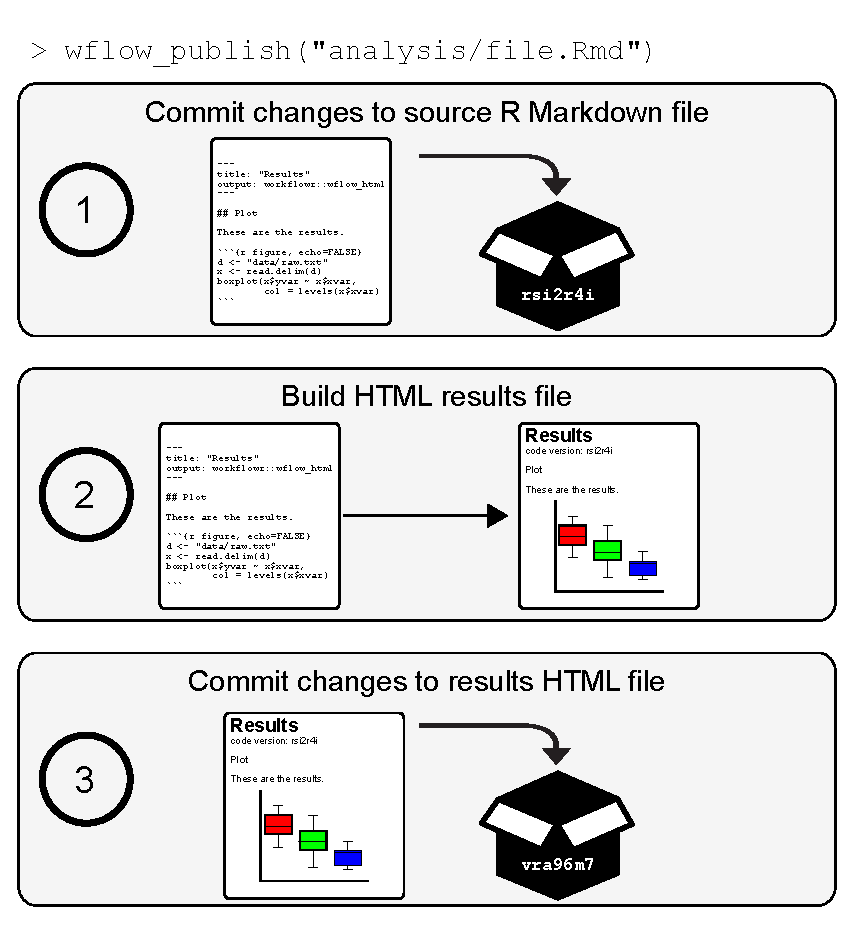
\includegraphics[width=0.8\textwidth]{figures/wflow-fig-2-v02.eps}

\cprotect\caption{\label{fig:publish}

The function \texttt{wflow\_publish()} simplifies and coordinates tracking of the
source code and results files with Git. The function performs a 3-step
procedure to ensure that the result HTML file is always created from a
unique and identifiable versioned Rmd analysis file. (1) The first step
commits the changes to Rmd analysisfile. (2) The second step builds the
results HTML file from the Rmd file. This ensures that the results were
generated from this exact version of the Rmd file. Furthermore, the
unique version of the Git repository is inserted directly into the HTML
file so that the source code used to generate the results is easily
identified and accessed. (3) The results HTML file (and any related
figure files) is committed to the Git repository. Thus, the versioning
of Rmd analysis files and corresponding HTML results files are
coordinated.

}

\end{figure}

Publishing an analysis is not final --- after calling \texttt{wflow\_publish()},
the analysis can be repeatedly updated and re-published using
\texttt{wflow\_publish()}. Each time \texttt{wflow\_publish()} succeeds in committing a new
version of the code and results, a link to previously published versions
of the analysis are embedded in the webpage so that readers can easily
access previous versions and compare with the latest results.

\subsubsection*{Checking in on the project's development: \texttt{wflow\_status()}}

As a workflowr project grows, it is important to be able to get an
overview of the project's status and identify files that may need
attention. This functionality is provided by the \texttt{wflow\_status()} command,
which gives the status of each Rmd file in the project -- either
“scratch”, “unpublished”, or “published”, whose definitions are given in
Figure \ref{fig:versioned}. The “published” Rmd files, which are those that have been run
through \texttt{wflow\_publish()}, are further recorded as either “up-to-date” or
“modified” depending on whether the Rmd file has been modified since
\texttt{wflow\_publish()} was run.

The \texttt{wflow\_status()} function highlights all Rmd files in the ``scratch'',
``unpublished'' or ``modified'' states and suggests suitable next
steps..



\begin{figure}

\# Figure \ref{fig:versioned}

\centering

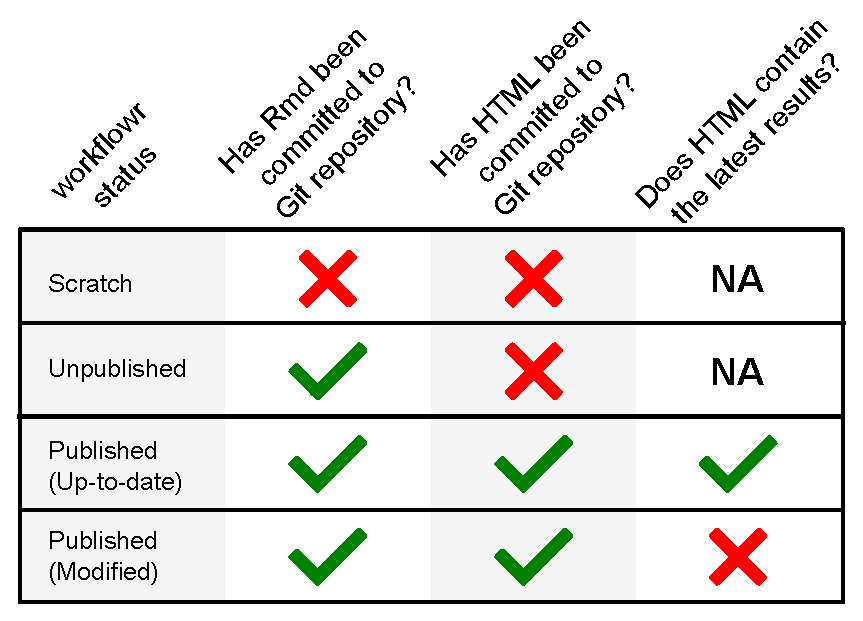
\includegraphics[width=0.8\textwidth]{figures/wflow-fig-3-v02.eps}

\cprotect\caption{\label{fig:versioned}

The workflowr package is an R Markdown -aware version control system.
The function \texttt{wflow\_status()} assigns a state to each Rmd file in the
workflowr project based on its status in the Git repository's working
tree, and based on the Git status of the corresponding HTML results
file.

}

\end{figure}



\begin{figure}

\# Figure \ref{fig:reproducible}

\centering

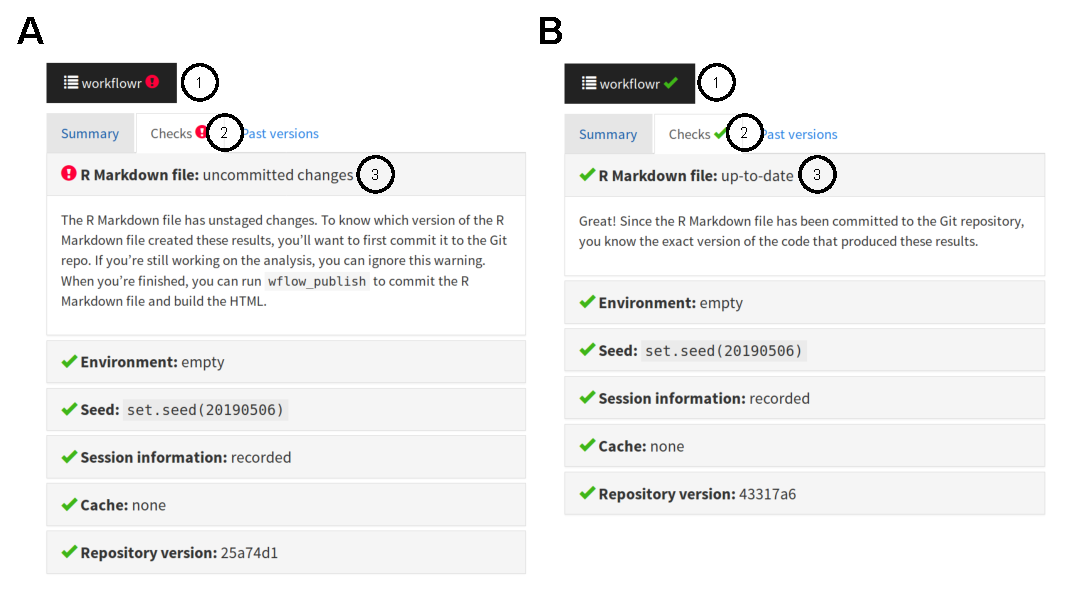
\includegraphics[width=0.8\textwidth]{figures/wflow-fig-4-v01.eps}

\cprotect\caption{\label{fig:reproducible}

The workflowr report summarizes the reproducibility checks inside the
results webpage. (A) A button is added to the top of each webpage.
Clicking on the button (1) reveals the full workflowr report with
multiple tabs. If any of the reproducibility checks have failed, a red
warning symbol (!) is shown. Clicking on the "Checks" tab (2) summarizes
the reproducibility checks, with icons next to each check indicating a
pass or failure. Clicking on an individual item (3) reveals a more
detailed description of the reproducibility check, with an explanation
of why it passed or failed. In (A), the Rmd file contains changes that
have not yet been committed, failing one of the reproducibility checks.
(Uncommitted changes are acceptable during active development, but not
acceptable when results are disseminated.) In this case, a
recommendation is given to run \texttt{wflow\_publish()} to fix the issue. (B) If
all the workflowr reproducibility checks pass, the workflowr button
shows a green checkmark (\CheckmarkBold), and clicking the individual
reproducibility checks (3) explains the importance of the check.

}

\end{figure}

\subsubsection*{Sharing code and results: \texttt{wflow\_git\_push()}}

The version-controlled website created by workflowr is self-contained,
so it can be hosted by most Web servers with little effort. Once the
website is available online, the code and results can be shared with
collaborators and colleagues by providing them with the website's URL.
Similarly, the workflowr repository can also serve as a companion
resource for a manuscript by referencing the website URL in the paper.

Since a workflowr project is also a Git repository, the most convenient
way to make the website available online is to use a Git hosting
service. The workflowr package includes functions \texttt{wflow\_use\_github()} and
\texttt{wflow\_use\_gitlab()} to simplify this process on two of the most widely
used services, GitHub and GitLab. Once a user has created a Git
repository on one of these online platforms, the project can be easily
uploaded using \texttt{wflow\_git\_push()}. (There is also a companion function
\texttt{wflow\_git\_pull()} for use when multiple people are collaborating on a
workflowr project, or when project is being updated from multiple
computers.)

The workflowr website results files include links to past versions of
analysis and figures, making it easy for collaborators to benefit from
the versioning of analyses without knowing anything about Git. For
example, if a collaborator would like to download a previous version of
a figure generated several months ago, this can be done by navigating
html links on the workflowr website.

\subsubsection*{Installation}

The workflowr software is available on CRAN, works with R versions 2.3.5
or later, and can be installed on any major platform that is supported
by R (Linux, macOS, Windows). It is regularly tested on all major
operating systems via several Continuous Integration services (AppVeyor,
CircleCI, Travis CI). It is also regularly tested by CRAN using machines
running Debian GNU/Linux, Fedora, macOS, Solaris and Windows.

Because workflowr uses the rmarkdown package to build the HTML pages, it
requires the document conversion software pandoc to be installed. The
easiest way for R users to install pandoc is to install RStudio.
Installing Git is not required because the R package dependency git2r
includes libgit2, a minimal Git implementation, but may be useful for
occasional management of the Git repository outside regular workflowr
usage.

\subsubsection*{Customization}

We designed workflowr projects to be highly customizable. For example,
the look of the webpages can be customized via options provided by the
rmarkdown package. These options can be customized in the
\verb|analysis/_site.yml| configuration file. Additional settings
specific to workflowr, such as setting the seed for the pseudorandom
number generation, or setting the working directory for the Rmd files,
can be controlled in the \verb|_workflowr.yml| file.

\subsection*{Implementation}

Here we give an overview of the workflowr package implementation. All workflowr commands can be invoked from R (or RStudio) so long as the working directory in R is set to the directory containing a workflowr project, or any subdirectory of a workflowr project (this is similar to how Git commands are invoked). To determine the workflowr project from a subdirectory, whenever a command is called from the R console, workflowr searches for the RStudio project file stored at the root of the project. This search is implemented using the rprojroot R package. (The RStudio project file is a required file, so if this file is deleted, the workflowr commands will fail.)

\subsubsection*{Organizing the project: \texttt{wflow\_start()}}

The function \texttt{wflow\_start()} populates the project directory using
predefined template files. It uses the glue R package to insert relevant
variables, e.g., the name of the project, directly into the newly
created files.

\subsubsection*{Generating results reproducibly: \texttt{wflow\_build()}}

The \texttt{wflow\_build()} function generates a responsive website from a
collection of Rmd files. It builds on the \texttt{render\_site()} function from
the rmarkdown package. Function \texttt{render\_site()} in turn builds on the
Bootstrap framework to create a responsive website with a navigation
bar. This includes downloading and linking to the required CSS and
JavaScript files. The website settings, such as the labels and URLs
included in the navigation bar, can be adjusted in the
\verb|analysis/_site.yml|configuration file. Like other R packages such
as bookdown that extend rmarkdown, workflowr provides a custom site
generator in function \texttt{wflow\_site()} that alters the website generation
process. For example, one change to this process is that the generated
website files (HTML, CSS, JavaScript) are moved instead of copied from
\verb|analysis/| to \verb|docs/|, which . This reduces unnecessary
duplication of files.

In the rmarkdown package, the rendering of webpages from Rmd files is
controlled by the function \texttt{html\_document()}. Workflowr provides an
analogous function, \texttt{wflow\_html()}, which extends \texttt{html\_document()}, and
allows for customization of the and the reproducibility checks.
Therefore, all features implemented in rmarkdown (e.g., code chunk
folding, generating a table of contents from the section headings) are
inherited by \texttt{wflow\_html()}.

Most of the workflowr content is added as a preprocessing step prior to
executing the R code in the Rmd file. To do this, \texttt{wflow\_html()} copies
the original Rmd file to a temporary directory, adds the additional
content, then executes the code. The content embedded into the R
Markdown includes code chunks such as R code at the start of the file
that calls \texttt{set.seed()} and R code toward the end of the file that calls
\texttt{sessionInfo()}, and inline HTML for elements such as the workflowr report
and links to previous versions of figures. There is also a brief
postprocessing step to incorporate additional HTML, CSS and JavaScript
elements needed to display the workflowr elements added in the
preprocessing step. This postprocessing is done when pandoc converts the
generated markdown to the final webpage.

The process for embedding links to past versions of files --- that is,
files added to previous commits in a Git repository --- requires some
additional explanation. Links to past versions are only included if the
user has set up a remote repository hosted by GitHub and GitLab.
Clicking a link to a past version of an Rmd file (or figure file) in a
Web browser will load a webpage displaying the R Markdown source code
(or figure file) as it is saved in the given commit. For past versions
of the webpages, we use an independent service raw.githack.com, which
displays the HTML file in the browser like any other webpage (this is
because GitHub and GitLab only show the raw HTML code).

The settings in \verb|analysis/_site.yml| are passed to function
\texttt{html\_document()} in the rmarkdown package. The settings in
\verb|_workflowr.yml| are read by \texttt{wflow\_html()}; see
\texttt{help(wflow\_html)} for a full documentation on all workflowr
settings that can be customized in this file. For example, the default
function used to record the session information at the bottom of each
webpage, \texttt{sessionInfo()}, can be overridden by adding the YAML field
\verb|sessioninfo| (e.g., the function from the devtools package could
be used instead by setting \verb|sessioninfo: devtools::session_info()|.

\texttt{wflow\_build()} creates a new R session to execute the code. This is
implemented using the R package callr. The workflowr package can be
configured to execute the Rmd files in a different directory from where
they are saved. This execution directory is controlled by the rmarkdown
option \verb|knit_root_dir|, which is set in \verb| _workflowr.yml| and
read by \texttt{wflow\_html()} before executing the code. By default, new projects
execute the R Markdown code chunks in the root directory.

\subsubsection*{Keeping track of the project's development: \texttt{wflow\_publish()}}

The workflowr functions use the R package git2r to run Git commands. The
git2r package is a wrapper around libgit2, a minimal C implementation of
Git.

This sequence of Git commands, and other operations, are executed behind
the scenes so that the user need only make a simple call to
\texttt{wflow\_publish()}. We have also implemented many checks and extensive
error handling to make sure that the Git repository and R environment
are in an acceptable state for committing the results. And when there
are issues that prevent committing of results workflowr provides
guidance on how to fix them.

\subsubsection*{Checking in on the project's development: \texttt{wflow\_status()}}

The \texttt{wflow\_status()} function checks the status of each Rmd file in the
project by comparing the state of the file in the Git repository's
working tree against the Git status of the corresponding HTML file. In
Git terminology, a “scratch” Rmd file in a workflowr project is an
uncommitted file in a Git repository; “unpublished” means that the Rmd
file is committed to the Git repository but the corresponding HTML is
not; a "published" Rmd file and its HTML file are both committed to the
Git repository; and a "modified" Rmd file has changes --- these changes
can be unstaged, staged, or committed --- that were made since the last
time the corresponding HTML file was committed (Figure \ref{fig:versioned}).

\subsubsection*{Sharing the code and results: \texttt{wflow\_git\_push()}}

To use \texttt{wflow\_git\_push()}, the remote Git repository must first be
configured. The user can configure the remotes manually using the git
remote subcommand or using \texttt{wflow\_git\_remote()}. Alternatively, the
workflowr package provides two functions, \texttt{wflow\_use\_github()} and
\texttt{wflow\_use\_gitlab()}, to simplify the creation and configuration of remote
repositories hosted on GitHub and GitLab. These two convenience
functions also add a navigation bar link with the URL of the remote
source code repository. The \texttt{wflow\_use\_gitlab()} function takes the
additional setup of activating the GitLab Pages by creating a file
.gitlab-ci.yml with the proper configuration. (GitHub Pages must be set
up manually because there is currently no way to do this automatically
via the GitHub API.).

\subsubsection*{Installation of workflowr and software dependencies}

Distribution and installation of the workflowr package is managed by the
Comprehensive R Archive Network (CRAN). The one software requirement
that is not automatically installed on most systems is pandoc.
Fortunately, pandoc comes bundled with RStudio, so users do not need to
install pandoc separately as long as they install workflowr from
RStudio. Alternatively, if R is used instead of RStudio, pandoc is
available for download via popular package managers such as Homebrew and
Anaconda. Users do not need to install Git; workflowr uses the
cross-platform C library libgit2, which is interfaced to R via the R
package git2r.


\section*{Use cases}

workflowr was officially released on CRAN in April 2018. As of July
2019, it has been downloaded from CRAN over 7,000 times, and it has been
adopted by many researchers to collaborate on research projects and
develop project websites to accompany research papers. Here we highlight
some successful examples.

\subsection*{Repositories for research projects}

\textbf{Human dermal fibroblast clonality project}

\url{https://davismcc.github.io/fibroblast-clonality}

A workflowr project accompanying a scientific paper on computational
methods for decoding the clonal substructures of somatic tissues from
DNA sequencing data \cite{McCarthy2018}. The webpages describe how to
reproduce the data processing and analysis, along with the outputs and
plots obtained by running the code.

\textbf{Characterizing and inferring quantitative cell cycle phase in
single-cell RNA-seq data analysis}

\url{https://github.com/jdblischak/fucci-seq}

A workflowr project supporting a paper on measuring cell cycle phase and
gene expression levels in human induced pluripotent stem cells
\cite{Hsiao2019}. The repository contains the processed data and code
implementing the analyses, and the full results can be browsed in the
website.

\textbf{Flexible statistical methods for estimating and testing effects
in genomic studies with multiple conditions}

\url{https://github.com/stephenslab/gtexresults}

A workflowr project containing the code and data used to produce the
results on the GTEx data set that were presented in \cite{Urbut2018}.

\textbf{Investigations on "truncated adaptive shrinkage"}

\url{https://github.com/LSun/truncash}

A workflowr project a Ph.D. student created to keep track of his
investigations into controlling false discoveries in the presence of
correlation and heteroskedastic noise. This repository illustrates the
use of workflowr as a scientific notebook --- the webpages contain
written notes, mathematical equations, source code, and the outputs
generated from running the code.

\subsection*{Repositories for courses}

\textbf{Stanford STATS 141—Biostatistics}

\url{https://xiangzhu.github.io/stanford-stats141}

A workflowr website for the Biostatistics course taught at Stanford. The
website includes working R examples, homework, the course syllabus and
other course materials.

\textbf{Single-cell RNA-seq workshop}

\url{https://github.com/crazyhottommy/scRNA-seq-workshop-Fall-2019}

A workflowr website for a workshop on analysis of single-cell RNA-seq
data offered by the Harvard Faculty of Arts and Sciences Informatics
group as part of a two-week long bioinformatics course. The R examples
demonstrate use of several bioinformatics packages such as Seurat and
msigdbr for preparation and analysis of single-cell RNA-seq data sets.

\textbf{Introduction to GIS in R}

\url{https://github.com/annakrystalli/intro-r-gis}

A workflowr website for a workshop given at the 2018 Evolutionary
Biology Conference. The website includes working R demonstrations, setup
instructions, and exercises.

\section*{Summary}

Our main aim in developing workflowr is to lower barriers to open and
reproducible code. The R package is straightforward to install, easy to
learn, and highly customizable.

The core functionality has been stable and will continue to be. In the
future, we plan to implement the following enhancements:

\begin{itemize}

\item Provide documentation and helper functions to support hosting the
workflowr website on additional platforms. Because it is a static
website, it could be hosted on many different platforms such as Netlify,
Heroku, etc.

\item Create a centralized website for registering and sharing workflowr
projects. In order to better promote open science, we would like to make
it easier for other interested researchers to discover existing
workflowr projects.

\item Implement basic support for small pipelines, including management
of code and file dependencies. Currently the only way to have workflowr
execute Rmd files in a specific order is to name them in alphanumeric
order. In the future, we plan to make it possible to specify which Rmd
files depend on each other. However, since it will still be focused only
on Rmd files, users will still be encouraged to use dedicated pipeline
software to build complex data analysis pipelines.

\end{itemize}

While workflowr aims to facilitate reproducible research, it is of
course not foolproof. Major limitations include 1) versioning of large
data files, 2) managing the computational environment, and 3) willful
tampering. The workflowr package ensures that each HTML results file was
created from a specific, known version of the corresponding Rmd file,
which is critical for reproducibility. However, if any imported data
files are not versioned by Git (or are out-of-date), then the results
will not be reproducible. This is mainly an issue for large data files.
Users are recommended to use Git LFS or similar software to version
large data files. Managing software dependencies is complex, and there
exist many solutions ranging from language-specific package managers
(e.g. packrat) to operating-system-level virtualization (e.g. Docker).
Instead of prescribing one solution over others, the workflowr package
simply records the session information that produces each result, and
otherwise leaves each user to decide how best to manage this complexity.
Lastly, the development history recorded by Git can be edited. Thus
while useful for transparency, it cannot be considered an immutable
record (e.g. like that provided by a blockchain).


\section*{Data availability}

Not applicable.


\section*{Software availability}

The workflowr software is open source and available from these URLs:

\begin{enumerate}

\item CRAN: \url{https://cran.r-project.org/package=workflowr}

\item Source code: \url{https://github.com/jdblischak/workflowr}

\item Documentation and tutorials:
\url{https://jdblischak.github.io/workflowr/}

\item Zenodo: \url{https://zenodo.org/badge/latestdoi/75893305}

\item License: \href{https://choosealicense.com/licenses/mit}{MIT}

\end{enumerate}


\section*{Author Contributions}

JDB: Conceptualization, Software, Writing – Original Draft Preparation,
Writing – Review \& Editing

PC: Software, Writing – Original Draft Preparation, Writing – Review \&
Editing

MS: Conceptualization, Funding Acquisition, Supervision, Writing –
Original Draft Preparation, Writing – Review \& Editing


\section*{Competing interests}

No competing interests were disclosed.


\section*{Grant information}

This work was supported by the Gordon and Betty Moore Foundation [Grant
number \#4559].

The funders had no role in study design, data collection and analysis,
decision to publish, or preparation of the manuscript.


\section*{Acknowledgments}

We thank the workflowr
\href{https://github.com/jdblischak/workflowr/graphs/contributors}{contributors}
for helping improve the package. We are also grateful for the many
workflowr users for testing the package and providing feedback---thanks
especially to \href{https://github.com/LSun}{Lei Sun},
\href{https://github.com/xiangzhu}{Xiang Zhu},
\href{https://github.com/NKweiwang}{Wei Wang}, and many other members of
the Stephens lab, past and present. We also acknowledge the authors and
contributors of the many great open source packages that the workflowr
package builds on. R packages particularly critical to workflowr's
implementation are
\href{https://cran.r-project.org/web/packages/git2r/index.html}{git2r},
\href{https://github.com/yihui/knitr}{knitr} and
\href{http://rmarkdown.rstudio.com/}{rmarkdown}.

{\small\bibliographystyle{unsrtnat}

\bibliography{references}}

\end{document}
